\documentclass[a4paper,11pt]{article}

\usepackage[utf8]{inputenc}
\usepackage[T1]{fontenc}
\usepackage[spanish]{babel}
\usepackage[pdftex]{graphicx}
\usepackage[hyphens]{url}
\usepackage[pdftex]{hyperref}
\hypersetup{
	pdftitle={Reglamento Laberinto},	% title
	pdfauthor={Club de Robótica FIUBA},	% author
	pdfsubject={Club de Robótica FIUBA},	% subject of the document
	colorlinks=true,		% false: boxed links;
	citecolor=black,		% color of links to bibliography
	filecolor=black,		% color of file links
	linkcolor=black,		% color of internal links
	urlcolor=black			% color of external links
}

%\usepackage{iwona}
\parskip=3pt
\headheight = 62pt

\usepackage{anysize}
%\marginsize{izquierdo}{derecho}{superior}{inferior}
\marginsize{2cm}{2cm}{1cm}{1cm}


\usepackage{fancyhdr}
\usepackage{lastpage}

%\fancyhf{} % clear all header and footer fields
\fancypagestyle{plain}{%
\fancyhead{} % get rid of headers
\renewcommand{\headrulewidth}{1pt} % and the line
\lhead{
\includegraphics[height=2cm]{logoclub.png}}
%\chead{}
\rhead{
\includegraphics[height=2cm]{logofiuba.jpg}}
\lfoot{ www.clubderobotica.com.ar}
\cfoot{}
\rfoot{ \thepage \ de \pageref{LastPage}}
}

\pagestyle{plain}

\let\oldenumerate\enumerate
\renewcommand{\enumerate}{
  \oldenumerate
  \setlength{\itemsep}{1pt}
  \setlength{\parskip}{0pt}
  \setlength{\parsep}{0pt}
}


\let\olditemize\itemize
\renewcommand{\itemize}{
  \olditemize
  \setlength{\itemsep}{1pt}
  \setlength{\parskip}{0pt}
  \setlength{\parsep}{0pt}
}


\newcommand{\cm}{\ensuremath{\mbox{~cm}}}


\author{Club de Robótica \\ Facultad de Ingeniería \\ Universidad de Buenos Aires}
\title{Competencia de Robótica 2014}


\begin{document}


\begin{center}
  {\Huge \textbf{Club de Robótica FIUBA}}
  \vspace{0.5cm}

  {\huge Competencia de Robótica 2014}
\end{center}

\section*{Objetivo de la competencia ``Laberinto''}
El objetivo de la competencia es diseñar y construir un robot autónomo capaz de encontrar la salida de un laberinto.
\section*{Organización}
\subsection*{General}
\begin{itemize}
  \item La organización se reserva el derecho de introducir cualquier cambio en la normativa, cuando lo estime oportuno para el desarrollo de las pruebas.
  \item El jurado se conformará de 3 personas seleccionadas por los organizadores de la competencia.
  \item Las decisiones de los jueces serán, en todo momento, inapelables.
  \item Pueden participar de esta competencia cualquier persona interesada. De ser menor de 18 años debe asistir acompañado por un mayor responsable.
  \item Los organizadores se reservan el derecho de admisión. En caso de conductas inapropiadas, a criterio del jurado, los organizadores podrán excluir a los equipos involucrados.
\end{itemize}

\subsection*{Inscripción}
\begin{itemize}
  \item Cada robot podrá ser registrado (a través del formulario correspondiente) por un equipo de hasta 4 miembros.
  \item Cada robot llevará un nombre. En caso de que dos robots sean registrados con el mismo nombre, la prioridad está determinada por el orden de pre-inscripción. Los restantes equipos podrán seleccionar otro nombre, o simplemente agregar un identificador (por ejemplo: robot\_2).
  \item Cada equipo debe tener al menos 1 miembro mayor de 18 años, que será responsable por los miembros menores de edad que pueda tener el equipo.
  \item En el día de la competencia por la mañana será la confirmación de asistencia y verificación de robots (``inscripción definitiva''). Es obligatorio presentarse antes de la finalización de este período para ser incluido en el torneo. Una vez cerrada la inscripción definitiva, se arma el cronograma de la competencia y orden de turnos, con todos los inscriptos.
  \item El horario de cierre de la ``inscripción definitiva'' se definirá en los días previos a la competencia. El horario de comienzo de la competencia se determinará el día del evento.
  \item Una vez publicado el orden, cada equipo es responsable de estar presente en el momento que corresponda su turno para competir.
  \item Parte de la calificación obtenida por los robots consiste en la documentación de cada robot debe presentar (ver ``El robot'').\textbf{Esta documentación debe ser enviada hasta una semana antes de la competencia}, de forma tal que el jurado tenga el suficiente tiempo para evaluarla.
  \item Además, esta información será publicada luego de finalizar la competencia, con el objetivo de favorecer el aprendizaje y fomentar el desarrollo de nuevos robots. Al realizar la inscripción del robot, todos los miembros del equipo están aceptando este compromiso.
\end{itemize}

\section*{El robot}
\subsection*{Requerimientos mínimos que debe cumplir el robot:}
\begin{itemize}
  \item El robot no puede tener ningún tipo de material o elementos que puedan dañar el circuito.
  \item Cada robot debe tener un interruptor (switch) que permita detenerlo inmediatamente. El interruptor debe ser visible y accesible quedando a criterio de los jueces el cumplimiento de este requerimiento.
  \item El robot debe ser completamente autónomo, es decir, no podrá necesitar de ningún tipo de conexión o comunicación con el exterior para participar de la competencia. Sí está permitido que el robot transmita datos útiles para el análisis de su desempeño. En caso de ser solicitado por el jurado, el equipo deberá demostrar que el robot puede funcionar sin este enlace activado.
  \item El robot deberá utilizar baterías. Está prohibido el uso de cualquier tipo de combustible.
\end{itemize}

No hay más restricciones, se pueden usar kits de robótica, kits de electrónica, o diseños completamente propios.

Se puede utilizar cualquier procesador o circuito para controlar el auto. El mismo criterio se aplica a los sensores, donde cualquiera está permitido.

Si bien no existen limitaciones para las dimensiones del robot, se recomienda tener en cuenta las dimensiones del laberinto ya que, por ejemplo, un robot muy grande quizás no pueda girar adecuadamente en las esquinas (más allá que su tamaño sea menor al ancho del laberinto).


\subsection*{Documentación del robot}
Parte de la calificación del robot comprende la evaluación, por parte del jurado, de la documentación prevista por el equipo.
Dicha documentación debe incluir:
\begin{enumerate}
  \item Carátula: documento editable provisto por el Club (descargar en la página) 
  \item Introducción:
  \begin{itemize}
    \item Descripcion basica del funcionamiento del robot 
    \item Objetivos (simpleza, excelencia, económico, reciclado, repetible, etc.)
  \end{itemize}
  \item Mecánica:
  \begin{itemize}
    \item Descripción de la estructura mecánica
    \item Especificaciones técnicas (Tipo, potencia y rpm de los motores, fuente de alimentación, etc.)
  \end{itemize}
  \item Electrónica:
  \begin{itemize}
    \item Descripción del circuito y mención de los integrados utilizados
    \item Esquemático y/o PCB 
  \end{itemize}
  \item Programación:
  \begin{itemize}
    \item Método de programación y programador utilizado
    \item Descripción de la lógica del código y lenguaje utilizado 
  \end{itemize}
  \item Conclusiones: Conclusiones del trabajo, costo total del robot, posibles mejoras a implementar, alternativas consideradas, etc.
  \item Anexo:
  \begin{itemize}
    \item Mecánica: Diagrama y planos (Diagramas 3d, dibujos, fotos del ensamblaje y/o croquis)
    \item Electrónica: Diagrama en bloques (optativo)
    \item Programación: 
    \begin{enumerate}
      \item Código fuente (en caso de que sea analógico, especificarlo, y explicar como calibraron el robot)
      \item Diagrama de flujos (optativo)
    \end{enumerate}
  \end{itemize}
\end{enumerate}

Las descripciones deben ser breves y concisas. La documentación no debe exceder el límite de 6 hojas máximo sin contar el anexo. 

El formato del documento deberá ser: 

Hoja: A4, Letra: Arial, Tamaño: 11, Alineación: Justificada, Interlineado: Sencillo y Sangría: $0.5\cm$. 

Se deberá enviar el archivo en formato PDF.\\

Un jurado puede solicitar a algunos participantes hacer una breve exposición oral e informal de los diseños luego de finalizar la carrera, ante toda la audiencia.\\

El objetivo de publicar los diseños y solicitar las presentaciones orales es favorecer el aprendizaje de todos los concursantes, estudiando los diseños de los demás.\\

Al momento de la inscripción, los miembros del equipo aseguran que la información presentada es de su propiedad intelectual, y/o los debidos créditos fueron incluidos. También acuerdan ceder los derechos de publicación de la información a los organizadores del evento, siendo ésta debidamente referenciada (es decir, aceptan que la información sea publicada en la página del club de robótica, indicando quiénes son los autores).

\section*{El Laberinto}
\begin{itemize}
  \item El laberinto se conforma por un conjunto de celdas de $28.0\cm \times 28.0\cm$  ($\pm0.5\cm$).
  \item El cruce entre celdas tiene una separación de $25.5 \times 25.5\cm$ ($\pm0.5\cm$).
  \item El piso es negro de pintura mate sobre una tabla de madera fibrofácil.
  \item Las paredes son blancas, de pintura mate en madera fibrofácil, de $20\cm$ ($\pm1\cm$) de altura.
  \item Cada celda está demarcada por una línea blanca de $0.5\cm$ ($\pm0.1\cm$).
    \begin{center}
      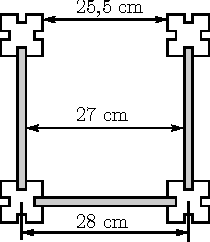
\includegraphics[width=0.3\textwidth]{paredes}
    \end{center}
  \item La salida es una celda de piso blanco, sin paredes.
\end{itemize}

El diseño del laberinto consiste en paredes móviles, lo que permitirá plantear varias configuraciones de laberinto.

\section*{La competencia}
\begin{itemize}
  \item Cada robot deberá completar una configuración del laberinto determinada por el jurado.
  \item Habrá dos rondas.
  \item En la primera ronda, de preclasificación, los robots deberán resolver un laberinto de $80\cm \times 160\cm$ ($3 \times 6$ celdas).
  \item Se ubica al robot en la celda y orientación iniciales, definidos por el jurado.
  \item El robot deberá alcanzar la celda blanca, considerada salida.
  \item Se considera que ha alcanzado la salida, cuando el robot se encuentre completamente sobre la celda blanca. No es necesario que el robot se detenga sobre esta celda.
  \item Los robots que completen exitosamente la primer ronda, participarán de la segunda ronda.
  \item En la segunda ronda se resolverá un laberinto de $160\cm \times 160\cm$ ($6 \times 6$ celdas).
  \item En esta segunda ronda se tomará el tiempo que le lleva al robot resolver el laberinto.
\end{itemize}


\subsection*{Formato}
\begin{itemize}
  \item Antes de la primera ronda, los equipos podrán hacer pruebas libremente sobre un laberinto.
  \item Al comienzo de la primera ronda los robots se deberán entregar al jurado, y no será posible programarlos hasta la finalización de la ronda.
  \item Una vez reunidos todos los robots, el jurado armará el laberinto a resolver.
  \item Luego de la finalización de la ronda, los equipos tendrán por lo menos 30 minutos para trabajar sobre el robot, pudiendo utilizar nuevamente el laberinto de pruebas.
  \item Para la segunda ronda se procederá de la misma forma.
\end{itemize}    

\subsubsection*{Primera Ronda}
\begin{itemize}
  \item Durante la primera ronda, el equipo puede detener el robot y volver a comenzar el laberinto, recordando que no puede modificar su programa.
  \item Cada robot dispondrá de 8 minutos como máximo.
\end{itemize}    

\subsubsection*{Segunda Ronda}
\begin{itemize}
  \item Durante la segunda ronda, el equipo tiene sólo dos intentos para resolver el laberinto. El objetivo es que el robot en la primera vuelta pueda, si lo desea, recorrer el laberinto, y encontrar el camino más corto hacia la salida. Por lo tanto se espera que en la segunda vuelta pueda resolver el laberinto más rápido.
  \item De cualquier forma se tomará el menor de los tiempos de cada intento.
  \item El tiempo sólo es válido si el robot logra llegar a la salida sin ayuda exterior.
  \item Si algún miembro del equipo interfiere con el robot durante alguno de los dos intentos, ese intento se anula sin asignar un tiempo válido y se le suma una penalidad al robot de 30 segundos para el tiempo que haga en el otro intento.
\end{itemize}    

\subsection*{Generales}
\begin{itemize}
  \item Si ningún equipo puede completar la primera ronda, el jurado puede proponer una configuración más simple.
Cada equipo es responsable de tener sus propias baterías y cargadores. Los equipos dispondrán de múltiples accesos a la red de energía eléctrica para cargar las baterías, pero no se otorgará tiempo extra para recargarlas cuando sean convocados a la pista, con lo cual es responsabilidad de cada grupo tener sus baterías cargadas.
\end{itemize}    

\subsection*{Puntuación}
Se calificará a los robots en tres categorías
\begin{enumerate}
  \item Resultado de la carrera (P1): se asignará un puntaje entre 0 y 10 puntos, según la siguiente escala:
  \begin{itemize}
    \item 10 puntos para el primero.
    \item  8 puntos para el segundo.
    \item  6 puntos para el tercero.
    \item  4 puntos para el cuarto.
    \item  2 puntos para los restantes robots que completaron una vuelta.
    \item  0 puntos para los que no completaron una vuelta del circuito.
  \end{itemize}    
    Se entiende por ``primero'' aquel robot que completa la vuelta en menor tiempo.

  \item Documentación (P2): El jurado calificará con una escala de 0 a 5 puntos la documentación presentada por cada equipo.
  A criterio del jurado se evaluará la calidad y completitud de todos los items indicados en la sección documentación.

  \item Originalidad del Robot (P3): El jurado calificará de 0 a 5 puntos según la originalidad que consideren de cada robot.
\end{enumerate}

Se dispondrá de una evaluación de cada jurado en relación a las categorías 2 y 3. Para cada una de estas categorías se promedian todos los puntajes otorgados por los jurado. Por ejemplo, para la categoría P2 se tendrán las notas de los 3 jurados. P2 se calcula como:

\begin{center}
P2=(J1+J2+J3)/3
\end{center}

La puntuación final del robot se obtiene con la siguiente ecuación:

\begin{center}
Puntaje final = P1 $\cdot$ $0.5$ + P2 $\cdot$ $0.7$ + P3 $\cdot$ 0,3
\end{center}

Está ecuación junto con las escalas seleccionadas otorga pesos a cada categoría de la siguiente forma:

1) 50\%  2) 35\%  3) 15\%

La puntuación máxima posible es 10 puntos.

\textbf{El ganador de la competencia es el robot que obtenga mayor cantidad de puntos}.

------------------------------------------------------------------------------------------

Este reglamento fue confeccionado por los miembros del Club de Robótica
\end{document}
